\chapter{Evaluation}
\label{chap:evaluation}

% "Moreover, under large record size (e.g., 1KB and above), B+ tree tend to have smaller write amplification than LSM-tree." - from "Closing the B+-tree vs. LSM-tree Write Amplification Gap on Modern Storage Hardware with Built-in Transparent Compression", Qiao et al., FAST 2022
% Good evaluation paper: https://dl.acm.org/doi/pdf/10.1145/3183713.3196895
% To adhere to the DAM model, can't we assume that all inner nodes are cached in memory, but leafs are not? see "A Comparison of Fractal Trees to Log-Structured Merge (LSM) Trees"

% - We reduce write amplification only if we write out a Delta Tree node with more than one entry since the last write-out.
% - If we always write out a Delta Tree node already after a single change, we do not benefit.

This chapter evaluates the performance and effectiveness of the proposed 3B-tree in reducing write amplification compared to traditional B-Trees. 
We describe the experimental setup (see \autoref{sec:experimental-setup}) and workloads (see \autoref{sec:workloads-datasets}) used, followed by an analysis of the results (see \autoref{sec:results-analysis}). 
The evaluation aims to quantify the trade-offs between write amplification (see \autoref{sec:write-amplification}), read amplification (see \autoref{sec:read-amplification}), space and memory overhead (see \autoref{sec:space_overhead} and \autoref{sec:in-memory-overhead}), and to demonstrate that the 3B-tree achieves significant \ac{IO} reductions while maintaining the desirable properties of conventional B-Trees.

\section{Experimental Setup}
\label{sec:experimental-setup}
Since we are interested in write amplification, we observe the number of page writes to disk for different workloads and different memory limitations.
This way, our results are not biased by the specific implementation, optimizations, and hardware that we run our experiments on.
All experiments were conducted locally on a Apple MacBook Pro with the specification listed in \autoref{tab:hardware-specs}.

\begin{table}[htbp]
\centering
\caption{Hardware Specifications}
\label{tab:hardware-specs}
\begin{tabular}{ll}
\toprule
\textbf{Component} & \textbf{Specification} \\ 
\midrule
Device & Apple MacBook Pro (2021) \\
Processor (CPU) & Apple M1 Pro (8-core, up to 3.2\,GHz) \\
GPU & Integrated 14-core Apple GPU \\
Memory (RAM) & 16\,GB \\
Storage & 512\,GB NVMe SSD \\
Operating System & macOS Sonoma 14.6.1 \\
\bottomrule
\end{tabular}
\end{table}

\section{Workloads and Datasets}
\label{sec:workloads-datasets}
We evaluate our approach on synthetic and real-world datasets.
The real-world dataset allows us to evaluate our approach on realistic data distributions and access patterns.
With the synthetic dataset, we can control the data distribution to evaluate the performance of our approach under different scenarios.
This allows us to identify the strengths and weaknesses of our approach.

We will be evaluating our system as a whole, benchmarking the database with the different indices to gain a holistic view of the performance.
To take a closer look at the indices themselves, we will also be benchmarking the indices in isolation, without the overhead of the database system.
For example, when benchmarking the whole database, we have to maintain the table data as well as the index, which introduces additional overhead.
When benchmarking the index in isolation, we can focus on the performance of the index itself.

\subsection*{Wikipedia Pageviews Workload}
We use an augmented Wikipedia Pageviews dataset \cite{wiki_pageviews} as a real-world dataset for our evaluation.
The primary goal of this dataset is to evaluate the performance of our approach on realistic data distributions and access patterns.
The dataset contains pageview statistics for all Wikipedia articles within a certain time frame.
It is publicly available and can be downloaded from the Wikimedia Dumps website\footnote{https://dumps.wikimedia.org/other/pageviews/}.
Each pageview record is of the form 
$$
\texttt{en Google\_Chrome 10406 0}
$$
consisting of the domain code, the page title, the number of views, and  the total response size in bytes.

\subsubsection*{Data Augmentation}
We use the hourly Pageview Wikipedia dataset from 1st of October 2025 at 00:00 UTC as our base dataset.
We augment the dataset in the following way:
\begin{enumerate}
    \item We filter out all non-English articles, i.e., we only keep articles with the domain code \texttt{en}.
    \item For benchmarks with integer keys, we turn the page title into an integer key. For benchmarks with variable-sized keys, we use the original page title as key.
    \item We create a lookup operation for each view of an article, i.e., if an article has 100 views, we create 100 lookups for that article.
    \item To generate a mixed workload, we turn a certain percentage of the lookups into updates. This assumes that an article with more views is more likely to be updated.
    \item We then shuffle the operations to create a mixed workload.
    \item To create a smaller dataset, we take a random fraction of the articles as samples.
\end{enumerate}

To populate the database, we insert all articles from filtered dataset once.
We then run the workload on the database or on the indices directly.

\subsubsection*{Workload Characteristics}
\label{sec:workload-characteristics}
The resulting workload has the following characteristics:
\begin{itemize}
    \item The dataset contains 59,240 distinct articles, translating to 59,240 distinct keys in the database.
    \item The workload contains 146,068 views in total.
    \item The keys follow a Zipf-like distribution, i.e. a small number articles are very popular and receive a large number of operations, while the majority of articles receive only a few. 
    \item In fact, 40,670 articles (\textasciitilde69\%) are viewed only once in the dataset. 
    The most viewed article, \textit{Jon\_Stewart}, received 2,998 views (\textasciitilde10\% of all views).
    \item \textbf{Update workload}: We transform 7,303 lookups into updates (\textasciitilde5\%) by default. When mentioned, we vary the update ratio from 0\% to 100\%.
    \item With an update ratio of 5\%, we update 5,724 distinct articles (\textasciitilde10\% of all articles) in the generated workload, whereas the majority of articles (\textasciitilde86\%) are only updated once.
    The most frequently updated article, \textit{Jon\_Stewart}, is updated 132 times (\textasciitilde10\% of all updates).
    \item \textbf{Insert workload}: To evaluate the performance of our approach on insert-heavy workloads, we create a workload with 100\% inserts as well.
    In this workload we insert all articles of the sample into an empty database or index.
    \item The keys are variable-sized strings with an average length of 20.5 characters, a maximum length of 236 characters and a minimum length of 1 character.
\end{itemize}

\section{Results and Analysis}
\label{sec:results-analysis}
In this section, we present the results of our benchmark experiments and analyze the performance of the B-tree and 3B-tree indices.
Our primary metric for this evaluation is the number of page writes to disk, which we aim to reduce.
To analyze the introduced read amplification, we also measure the total \ac{IO} operations (page reads + page writes) for both indices (see \autoref{sec:read-amplification}).

The goal of this evaluation is to determine whether the 3B-tree can reduce \ac{IO} operations compared to a traditional B-tree under different workloads and constraints and to understand the trade-offs involved in using a 3B-tree.

\subsection{Write Amplification}
\label{sec:write-amplification}
For a first analysis, we consider the write amplification of the B-tree and 3B-tree indices when running the mixed Wikipedia Pageviews workload with 5\% updates on the sample dataset.
For now, we run the workload on the indices directly without the overhead of the database system in the buffer.
% TODO: Check if this is still true:
To gain a holistic view of the performance, we will also run the workload on the whole database in \autoref{sec:database-evaluation}.
We benchmarked with 4 KB pages, a buffer pool of 400 pages (\textasciitilde80\% of the B-Tree pages), and a write threshold of 5\% (i.e. we only write pages to disk if >5\% of the page has been modified in the case of a 3B-tree index).
The base B-tree in both indices produce a tree with 502 nodes in total.
Both inner and leaf nodes fit 170 entries each, while the average node is filled to \textasciitilde70\%.
There is no difference in fanout between the two indices (see Space Overhead \ref{sec:space_overhead}).
We compare the number of page writes to disk for both indices.

The results are shown in \autoref{fig:page-writes-mixed}.
We observe a reduction of \textasciitilde69\% in total page writes when using the 3B-tree compared to the B-tree.
We can see, that in the 3B-tree index, the majority of page writes occur in the Delta Tree than its base B-Tree.
This shows that we successfully defer small writes across the B-tree and batch them more efficiently in fewer pages in the Delta Tree.

\begin{figure}[htbp]
  \centering
  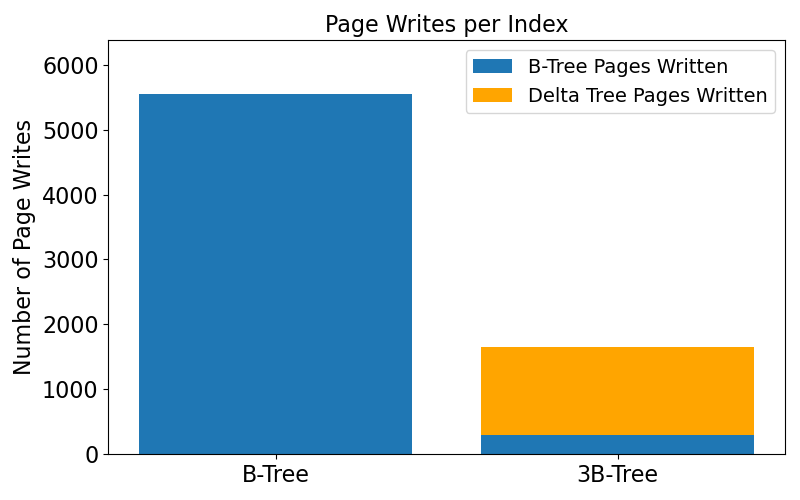
\includegraphics[width=0.6\textwidth]{figures/evaluation/pageviews_mixed_index.png}
  \caption{Running the mixed Wikipedia Pageviews workload with 5\% updates, 4 KB pages, a buffer pool of 400 pages (\textasciitilde80\% of the B-tree pages), and a write threshold of 5\%. We see a reduction of \textasciitilde69\% in page writes when using the 3B-tree compared to the B-tree.}
  \label{fig:page-writes-mixed}
\end{figure}

In the following sections, we analyze the performance of the 3B-tree under different scenarios and workloads to understand its strengths and weaknesses.

% TODO: Index as part of the database vs. index in isolation
% When running the workload on the database as a whole (\autoref{fig:sub1}), we see a reduction in page writes of \textasciitilde23\% when using the 3B-tree compared to the B-tree.
% When running the workload on the indices directly (\autoref{fig:sub2}), we see a more significant reduction in page writes of \textasciitilde66\% when using the 3B-tree compared to the B-tree.

% There are two main reasons for the difference in write amplification reduction between the two scenarios.
% \begin{enumerate}
%   \item \textbf{Relative Impact}: Firstly and more obviously, when running the workload on the database, we have more pages in the system that are not affected by our method.
% Our method effects a smaller fraction of the total number of pages in the buffer, therefore our relative impact is naturally smaller.
% When running the workload on the indices directly, we can focus on the performance of the method itself without the overhead of maintaining the table data.
% Therefore, we will focus on the results when running the workload on the indices in isolation in the following analysis.
%   \item \textbf{Memory Constraints}: More importantly, the indices have different memory constraints in the two scenarios.
% When running the workload on the database, the indices have to share the buffer pool with the table data.
% When running isolated, the indices can use the full memory available in the system. 
% In the metrics collected during the benchmark runs, we could see that we have 10-15\% higher buffer hit rates when running the workload on the indices directly.
% While both indices have the same memory available and higher buffer hit rates when running isolated, the 3B-tree performs better in terms of write amplification reduction.
% \end{enumerate}

% These findings indicate that the 3B-tree can significantly reduce write amplification compared to a traditional B-tree, especially when the index can effectively utilize the available memory.
% To investigate this further, we will run the workload under different memory constraints in the following section.

\subsubsection*{Different Memory Constraints}
To understand the impact of memory constraints on the performance of the 3B-tree, we run the same workload with different buffer pool sizes.
To repeat, the workload produces a B-tree of 502 pages in total. We vary the buffer pool size from 25 (\textasciitilde5\% of the B-tree) to 500 pages (\textasciitilde99\% of the B-tree), while keeping the page size at 4 KB and the write threshold at 5\%.
The results are shown in \autoref{fig:buffer_sizes}.

One key observation is that the 3B-tree degrades more smoothly with lowering memory capacities than the B-tree.
When the buffer pool size is reduced from 500 (99\%) to 400 pages (80\%), the B-tree experiences a sharp increase in page writes.
Further reductions in buffer pool size lead to smaller increases in page writes.
In contrast, the 3B-tree experiences a steady increase in page writes as the buffer pool size is reduced.

In the following, we analyze the performance of the 3B-tree under different memory constraints in more detail.
We differentiate between low (5\%-10\%), restricted (20\%-80\%) and high (>99\%) memory capacities.
Percentages are given with respect to the total number of B-tree pages.
Both indices produce the same amount of B-tree pages in all settings.

\begin{figure}[htbp]
  \centering
  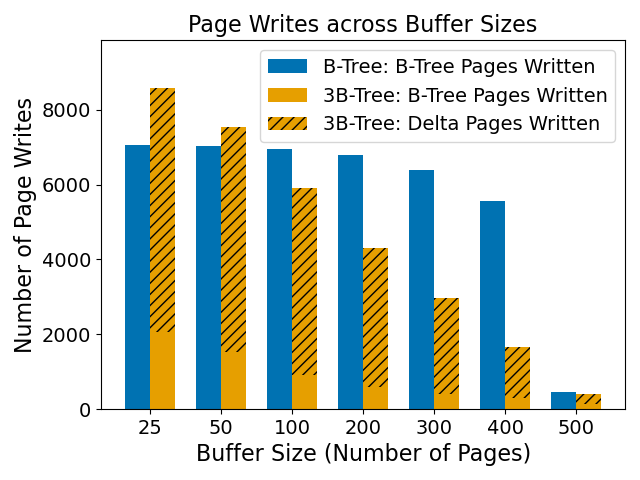
\includegraphics[width=0.6\textwidth]{figures/evaluation/pageviews_buffer_sizes.png}
  \caption{The impact of buffer pool sizes on the amount of page writes per index with a 4 KB page size and a 5\% write threshold.
  The B-tree in both indices has 502 pages to address the dataset.
  The 3B-tree requires enough memory to effectively batch changes in the Delta Tree and degrades more smoothly with lowering memory capacities than the B-tree.}
  \label{fig:buffer_sizes}
\end{figure}

\inlinesection{Low Memory Capacity.}
With a buffer pool of 25 to 50 pages, we can see an increase in page writes with the 3B-tree compared to the B-tree.
For example, with 25 buffer pool pages, the 3B-tree writes its B-tree pages 4,993 times less, but introduces 6,506 page writes in the Delta Tree.
Two questions arise:
\begin{enumerate}
  \item \textit{Why do we not reduce page writes?}
  When we do not have enough memory to cache pages, we cannot accumulate changes in the Delta Tree effectively.
  The Delta Tree improves page writes only when at least two changes can be accumulated on a Delta Tree page before writing it to disk again.
  The inserted deltas between page writes of the Delta Tree page must be $>1$ on average to see an improvement.
  When constantly swapping pages in and out of memory, we simply move the page write from one tree to another.
  Since the 3B-tree shares the buffer pool between two trees, memory is more constrained for each tree.
  This leads to more page traffic overall, further reducing the probability of accumulating changes in a Delta Tree leaf.
  \item \textit{Why do we have even more page writes?}
  When moving page writes from one tree to another, we would expect to see the same amount of page writes overall.
  The average amount of deltas inserted (i.e. B-tree page writes deferred) in between Delta Tree page writes should be equal to $1$.
  However, we see more page writes with the 3B-tree than with the standalone B-tree.
  The average amount of deltas inserted in between Delta Tree page writes is actually smaller than $1$ ($4,993 / 6,506 \approx 0.77$) with a buffer pool of 25 pages.
  This means we can dirty more Delta Tree pages than we inserted deltas. 
  Firstly, when inserting a delta we can trigger a split in the Delta Tree, causing a new inner node to be created or updated in the B-tree. 
  Secondly, we must delete entries from the Delta Tree when B-tree pages have accumulated enough changes to actually write them to disk.
\end{enumerate}

The 3B-tree cannot utilize its batching capabilities without caching.
In such a setting, we merely introduce further write amplification in the system since we have more pages to maintain.
The 3B-tree requires enough memory to accumulate changes over time.
Only with effective page caching, we can reduce the page writes in total.

\inlinesection{Restricted Memory Capacity.}
With limited memory capacities of 100-500 pages, we see a significant reduction in page writes with the 3B-tree compared to the B-tree.
The 3B-tree can reduce page writes up to \textasciitilde70\% compared to the standalone B-tree.
The larger the available memory, the more changes we can accumulate in our Delta Tree before writing them to disk.
For example, with a buffer pool of 400 pages, we can see that a Delta Tree page write accumulates 4 deltas on average before being written to disk.
We achieve the batching effect that we are aiming for, leading to fewer total page writes.
This shows that our method can effectively utilize the available memory to reduce write amplification in memory-constrained settings.

\inlinesection{High Memory Capacity.}
With a buffer pool of 500 pages, almost all pages can be kept in memory, therefore the effect is less pronounced.
With a buffer pool of 502 pages (100\% of the B-tree), we could hold the entire B-tree in memory.
The Delta Tree is obsolete in this setting, as we can keep all changes in memory without writing them to disk.
Since the Delta Tree is empty, and no B-tree pages are loaded from disk once they are in memory, we do not have to perform any lookups into the Delta Tree.
Therefore, the 3B-tree does not incur any overhead compared to the B-tree except from tracking changes in the B-tree nodes.
However, this overhead is negligible as shown in \autoref{sec:in-memory-overhead}.

\inlinesection{Summary.}
To summarize, the 3B-tree can reduce write amplification in memory-constrained settings where the entire dataset does not fit in memory.
This optimization is achievable only when enough memory is available for effective caching.
Enough memory must be available to accumulate changes in the Delta Tree over time.
An ideal buffer pool size is \textasciitilde20\%-80\% of the B-tree pages.
Across all memory constraints, the 3B-tree degrades more smoothly than the B-tree, making it a robust choice for varying memory conditions.

\subsubsection*{Different Write Thresholds}
\label{sec:different-write-thresholds}
To repeat, the write threshold defines the minimum percentage of a page that has to be modified before we write it to disk.
When it is smaller than the threshold, we buffer the changes in the Delta Tree and discard the page.
To understand the impact of the write threshold on the performance of the 3B-tree, we run the same workload with different write thresholds.
We fixate the page size at 4 KB and the buffer pool size at 400 pages (\textasciitilde80\% of the B-tree), as this setting showed the most significant improvements in the previous section.
We vary the write threshold from 0\% to 50\%.
Thresholds beyond 50\% are not meaningful, as Delta Tree would not be able to accumulate more than one change on leaf nodes.
The results are shown in \autoref{fig:write_thresholds}.
For the baseline B-tree index, the write threshold has no effect, as we always write every change to disk immediately.
Therefore, we show the results in percentage improvement of the 3B-tree page writes over the standalone B-tree.

Without buffering, at a write threshold of 0\%, we write every changed page to disk immediately, just as a traditional B-tree would.
As expected, we see no improvement in page writes in this setting.
In fact, we can have a few more page writes since we still buffer the empty root of the Delta Tree (it is still read when loading B-tree pages from storage), leaving slightly less memory for the B-tree pages.
Starting from a write threshold of 1\%, we can accumulate changes in the Delta Tree and reduce page writes by \textasciitilde70\% compared to the B-tree.

\begin{figure}[htbp]
  \centering
  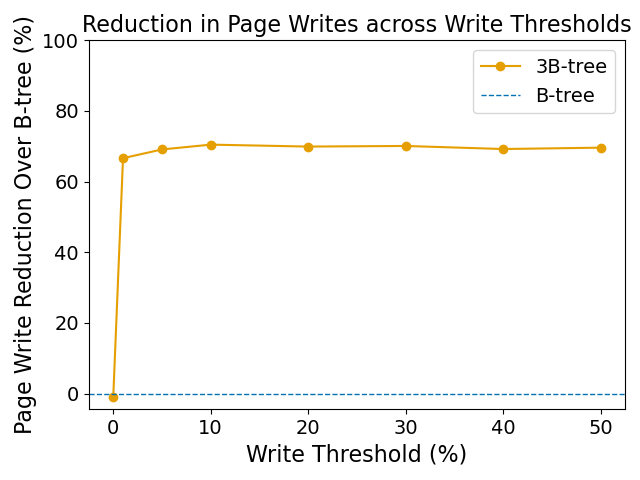
\includegraphics[width=0.6\textwidth]{figures/evaluation/pageviews_mixed_write_thresholds.png}
  \caption{The impact of different write thresholds on the amount of page writes per index when running the mixed workload with 5\% updates. The page writes of the B-tree index (marked in blue) are constant across all thresholds. The 3B-tree (marked in orange) page writes are shown in percentages of improvement over the B-Tree page writes. At 0\% threshold, we write every B-tree node to disk after every change, leading to no improvement in write amplification. With higher thresholds, we can accumulate changes before writing them to disk, leading to significantly fewer page writes.}
  \label{fig:write_thresholds}
\end{figure}

\inlinesection{Expected Diminishing Returns.}
We do not see a diminishing return with higher write thresholds, as expected.
We expected to see smaller improvements with larger write thresholds for three reasons:
\begin{enumerate}
\item \textbf{Fewer Changes Fit into a Page:} 
We achieve our goal of reducing page writes when we can accumulate changes on $y$ pages into a single page of the Delta Tree, where $y > 1$.
We can then save up to $y - 1$ page writes.
However, with larger write thresholds, fewer pages' changes fit into a single page.
For example, with a 1\% threshold, we can fit 100 pages' changes into a single 4 KB page, while with a 25\% threshold, we can only fit 4 pages' changes in the worst case.
The maximum accumulation factor $y$ decreases with larger write thresholds, leading to fewer potential savings in page writes.
\item \textbf{Less Likelihood to Batch Changes:}
With fewer changes fitting into a single page, the likelihood of batching changes in between Delta Tree page writes decreases.
For example, assume a Delta Tree node $d$ that holds $x$ delta arrays for $x$ B-tree nodes.
This means, at some point $x$ B-tree nodes have been modified. 
However, this does not directly translate to $x$ saved page writes, because $d$ itself might have been written to disk before all $x$ B-tree nodes were modified.
Therefore, we only batch changes that happen between two writes of $d$.
When $d$ holds the changes of 100 B-tree nodes, the likelihood of batching changes is much higher than when $d$ only holds the changes of 4 B-tree nodes.
On average, we can save $\frac{y - 1}{s}$ page writes per Delta Node $d$, where $s$ is the number of times $d$ has been written to disk.
\item \textbf{More Leaf Nodes in Delta Tree:}
Additionally, with larger deltas, we require more leaf nodes in the Delta Tree to address all changes.
This introduces more page overhead in the system, leading to more page traffic.
This increases $s$, the number of times a Delta Tree node is written to disk.
(The fanout itself is not affected, since inner nodes only hold fixed size \ac{PID}s as keys. The variable-sized deltas are only stored in the leaf nodes, so more pages need to be addressed by the Delta Tree.)
\end{enumerate}

\inlinesection{Stagnating Improvements.}
For all three reasons, we should see shrinking improvements, the larger the write threshold becomes.
However, the improvements we see more or less stagnate after a write threshold of 20\%.
The reason is that we do not see many pages that are modified more than 20\% between page writes.
In \autoref{tab:modification-degree}, we can see the distribution of the modification degree for all modified B-tree nodes at the time of eviction.
There are two reasons why we only see a small degree of change for most pages:

\begin{enumerate}
\item \textbf{Zipf-like Distribution:}
Due to the Zipf-like distribution of the keys in the workload, a small number of very popular articles receive a large number of operations, while the majority of articles receive only a few.
With an update ratio of 5\% of all operations in the workload, most articles are not updated at all (\textasciitilde 90\%).
Naturally, with updates scattered across the index, most pages are only slightly modified between page writes.
Therefore, we run the same experiment with a workload of 100\% insert to see if the improvements change.
The results are shown in \autoref{fig:write_thresholds_insert}.
The insertion workload distributes inserts more evenly across the index, as every article is inserted once.
The order of articles is shuffled, so we do not have any locality in the inserts.
Indeed we can observe the diminishing returns more clearly in this workload.
However, the improvements still stagnate after a write threshold of 20\%.
This workload introduces a lot of modification activity per page, therefore we would expect to see a more drastic reduction.
The reason is explained in the next point.
\item \textbf{Pages are Written Before They Reach High Degrees of Change:}
While investigating, we found that pages are often written to disk before they can accumulate many changes.
In \autoref{tab:modification-degree}, we can see the distribution of the modification degree for all modified B-tree nodes at the time their changes are stored in the Delta Tree.
We chose a write threshold of 100\% for this experiment to see the full distribution of modification degrees.
It only shows the pages that are inserted into the Delta Tree, not the pages that bypass the Delta Tree and are directly written to disk.
We can see that the Delta Tree only receives small deltas from the B-tree for the vast majority of nodes across workloads.
Even in a workload with 100\% inserts, where some nodes experience a lot of changes such as node splits, we see that they do not end up in the Delta Tree.
One reason is that \textbf{we write new pages to disk immediately} at eviction.
Another reason is that node splits combined with many inserts introduce \textbf{change degrees over 100\%} for a page, which is higher than the write threshold of 100\% and therefore is written to disk.
Lastly, we sometimes have to write B-tree nodes to disk even though their degree of change is below the write threshold.
Sometimes we have to lock the Delta Tree to protect against recursive evictions that want to modify the Delta Tree.
For example, when a B-tree node is evicted and its delta is inserted into the Delta Tree, this might cause a split in the Delta Tree.
The split causes a new node to be created, which has to be inserted into the B-tree.
In this moment, the Delta Tree is in an incomplete state and cannot be accessed by other operations.
However, the newly created node can trigger another eviction in the buffer manager, which might evict a modified B-tree node.
This modified B-tree node cannot insert its delta into the Delta Tree, as it is currently experiencing structure modifications and therefore is locked.
In such cases, \textbf{we force B-tree nodes to disk even though their degree of change is below the write threshold}.

While investigating, we observed that every B-tree node is forced to disk at least once during the workloads for one of these reasons.
Therefore, we never see high degrees of change for any page, as we write them to disk before they can accumulate more changes.
\end{enumerate}

\begin{figure}[htbp]
  \centering
  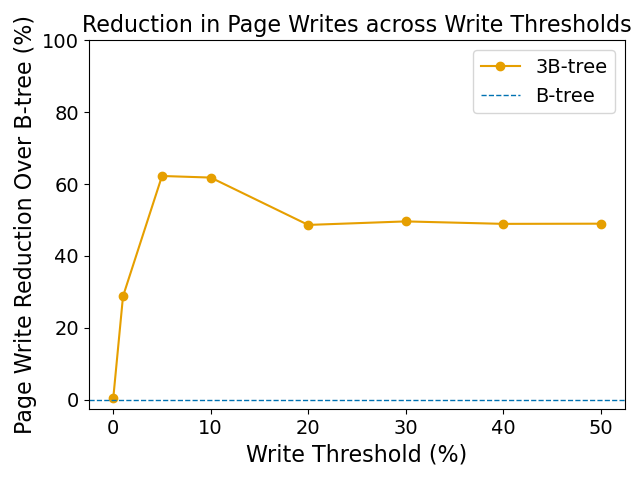
\includegraphics[width=0.6\textwidth]{figures/evaluation/pageviews_insert_write_thresholds.png}
  \caption{The impact of different write thresholds on the amount of page writes per index when running a workload with 100\% inserts. Similar to the mixed workload, we see significant improvements with small write thresholds that stagnate with larger thresholds. However, we can see a diminishing return as expected.}
  \label{fig:write_thresholds_insert}
\end{figure}

\begin{table}[ht]
  \centering
    \begin{tabular}{l|ccc}
    \toprule
    & \multicolumn{3}{c}{\textbf{Num. Pages}} \\
    \cmidrule(lr){2-4}
    \textbf{Modified} & \textbf{5\% Updates} & \textbf{100\% Updates} & \textbf{100\% Inserts} \\
    \midrule
    0--10\%   & 5274 &  38530 &  6462 \\
    10--20\%  & 670 & 1906 &  1892 \\
    20--30\%  & 1 & 61 & 586 \\
    30--40\%  & 0 & 1 & 129\\
    40--50\%  & 0 & 0 & 39 \\
    50--60\%  & 0 & 0 & 156 \\
    60--70\%  & 0 & 0 & 51 \\
    70--80\%  & 0 & 0 & 3 \\
    80--90\%  & 0 & 0 & 0 \\
    90--100\% & 0 & 0 & 0 \\
    $>$100\% & 0 & 0 & 0 \\
    \bottomrule
  \end{tabular}
  \caption{Distribution of B-tree pages by their modification degree (percentage intervals) when being unloaded to the Delta Tree with a Write Threshold of 100\% for different workloads. The majority of pages are only slightly modified between writes, even with a workload of 100\% inserts. Pages are unloaded to disk before they can accumulate more changes.}
  \label{tab:modification-degree}
\end{table}

A more sequential workload could help to increase the degree of change for pages that end up in the Delta Tree.
However, in such a scenario, traditional B-trees already perform very well.
Therefore, we cannot expect to see significant improvements with very high write thresholds in such a workload.

\inlinesection{Summary.}
Our method performs best with small write thresholds.
For higher thresholds, we expect diminishing returns due to fewer changes fitting into a page, less likelihood to batch changes, and more leaf nodes in the Delta Tree.
However, due to the workload characteristics and the eviction behavior of our implementation, we do not see high degrees of change for most pages.
The sweet spot for the write threshold is 5\%, where we can achieve significant reductions in page writes for different random write workloads (random updates and random inserts).
Therefore, we continue to use this setting in the following experiments.

\subsubsection*{Different Read/Write Ratios}
To understand the impact of different read/write ratios on the performance of the 3B-tree, we run the same workload with different update ratios.
We fixate the buffer pool size at 500 pages, the page size at 4 KB, and the write threshold at 5\%.
We vary the update ratio from 0\% to 100\%, i.e. we run workloads with only lookups, only updates, and mixed workloads in between.
The results are shown in \autoref{fig:write-ratios}.
We measure write amplification as the ratio of total bytes written to disk over the total bytes of the entries we modify in the index.

In a read-only workload we perform no page writes at all, as expected.
With writes present in the workload, we see a significant reduction in page writes with the 3B-tree compared to the B-tree.
The write amplification itself is higher for fewer updates, as we scatter small writes across the index, leading to more pages written for a small set of updates.
Here the 3B-tree can reduce write amplification by up to \textasciitilde70\% by batching them to fewer pages in the Delta Tree.
With more updates, more entries are modified in the same pages, leading to lower write amplification.
The 3B-tree can still reduce write amplification by \textasciitilde50\% in a workload with 100\% updates.
Even though we update every entry in the index with this workload, the 3B-tree can defer the page writes until more changes have accumulated, while the B-tree writes its pages to disk immediately upon eviction.

\begin{figure}[htpb]
  \centering
  \begin{subfigure}[t]{0.49\textwidth}
    \centering
    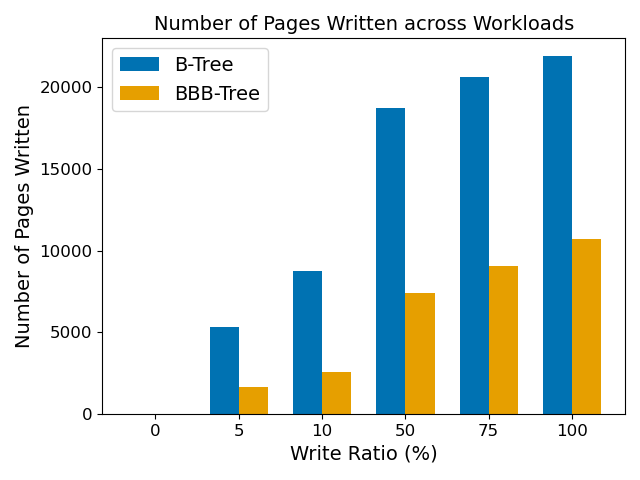
\includegraphics[width=\textwidth]{figures/evaluation/pageviews_write_ratios.png}
    \caption{Page Writes per workload.}
    \label{fig:write-ratios-page-writes}
  \end{subfigure}
  \hfill
  \begin{subfigure}[t]{0.49\textwidth}
    \centering
    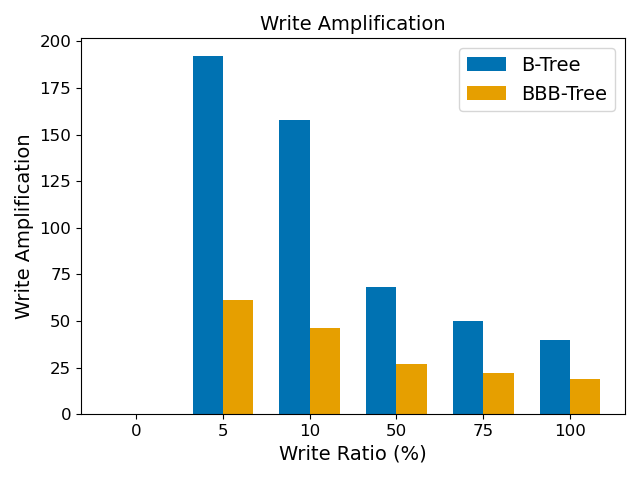
\includegraphics[width=\textwidth]{figures/evaluation/pageviews_write_ratios_wa.png}
    \caption{Write Amplification per workload.}
    \label{fig:write-ratios-wa}
  \end{subfigure}
  \caption{Page Writes and Write Amplification of the B-tree and 3B-tree with different write/read ratios in the workload. Without updates we have no page writes and therefore no write amplification. While page writes increase with more updates, write amplification decreases, as more changes happen in the same pages. The 3B-tree can reduce write amplification significantly across all workloads.}  
  \label{fig:write-ratios}
\end{figure}

\subsection{Read Amplification}
\label{sec:read-amplification}
Looking at page writes only does not give the full picture of the performance of the 3B-tree.
We need to consider the page reads as well to understand the overall \ac{IO} performance.
Therefore, we investigate the read amplification of the 3B-tree compared to a traditional B-tree.
To repeat, read amplification describes the amount of \ac{IO} operations we need to perform to answer a query (see \autoref{sec:read-amplification-background}).
However, for the purpose of this analysis, we specifically refer to \textbf{the ratio of page reads we add compared to the traditional B-tree}.
In addition to the page writes we save, we analyze the total amount of \ac{IO} operations, i.e., the read amplification.

\inlinesection{Additional Page Reads.} 
We introduce additional page reads in the following way:
\begin{enumerate}
  \item Every time we load a B-tree page from disk, we have to look up the \ac{PID} in the Delta Tree for any changes that need to be applied.
  \item Every time we unload a B-tree's dirty page, we either delete its deltas from the Delta Tree (if the page is written to disk) or insert/update its deltas in the Delta Tree (if the page is not written to disk).
\end{enumerate}
All these operations require a traversal through the Delta Tree, loading nodes from disk, if they are not in memory.
Additionally, sharing the buffer pool between two trees leads to more page traffic in both trees.
We show the sources of additional page reads in the following.

\inlinesection{Buffer Pool Analysis.}
To analyze the introduced page reads, we collect the buffer hits and misses per index under varying buffer sizes on the mixed workload with 5\% updates.
We show the misses and hits caused by the underlying B-trees and the Delta Tree separately.
Each buffer miss directly translates to a page read from disk.
The results are illustrated in \autoref{fig:buffer-traffic}.
We can observe the two sources of additional page reads (buffer misses) for the 3B-tree:
\begin{enumerate}
  \item \textbf{More B-tree Misses:} 
  The 3B-tree has more buffer misses for B-tree accesses compared to the standalone B-tree.
  Since the buffer pool is shared between the two trees, the 3B-tree has slightly less space to cache B-tree pages, leading to more buffer misses for B-tree accesses.
  However, the difference is similar across different buffer sizes.
  \item \textbf{Delta Tree Misses:} 
  The 3B-tree has additional buffer accesses for the Delta Tree.
  While most of these accesses result in buffer hits with enough memory available, we still have some buffer misses that lead to additional page reads.
  With small buffer sizes, the B-tree has more page swaps and therefore, the Delta Tree is accessed more frequently, leading to more total buffer accesses (hits and misses).
\end{enumerate}

The key observation is that reads are mostly amplified due to the Delta Tree's buffer misses.
Therefore, caching the Delta Tree effectively is critical to keep additional page reads low.

\begin{figure}[htpb]
  \centering
  \begin{subfigure}[t]{0.49\textwidth}
    \centering
    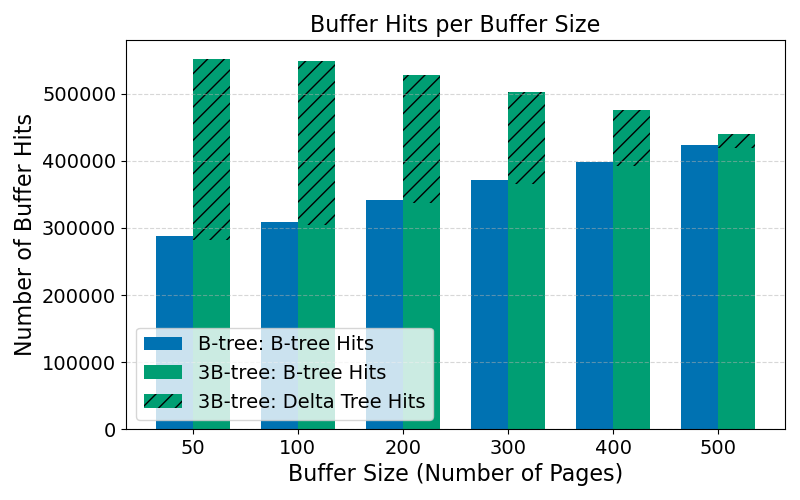
\includegraphics[width=\textwidth]{figures/evaluation/buffer_hits_per_buffer_size.png}
    \caption{Buffer Hits}
  \end{subfigure}
  \hfill
  \begin{subfigure}[t]{0.49\textwidth}
    \centering
    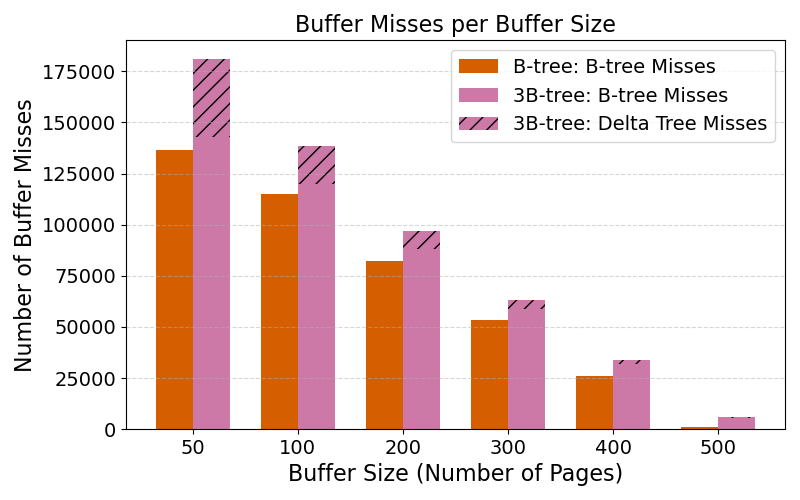
\includegraphics[width=\textwidth]{figures/evaluation/buffer_misses_per_buffer_size.png}
    \caption{Buffer Misses}
  \end{subfigure}
  \caption{Buffer hits and misses per index across different buffer sizes, separated into B-tree accesses and Delta Tree accesses. We used a page size of 4 KB, a write threshold of 5\% and a mixed workload with 4\% updates. The B-tree needs 502 pages to address the dataset in all cases.}
  \label{fig:buffer-traffic}
\end{figure}

\inlinesection{Buffer Size.}
The smallest amount of page reads is introduced with a buffer size of 200 pages (\textasciitilde40\% of the B-tree), where we only introduce \textasciitilde17\% more reads compared to the baseline B-tree.
We therefore use this buffer size in the following analysis of total \ac{IO} operations.
While higher buffer sizes (300-400 pages) lead to more savings in write amplification (see \autoref{fig:buffer_sizes}), we prioritize the reduction of reads, since we perform more reads than writes overall.

\inlinesection{Delta Tree Size.}
If we can cache most of the Delta Tree pages, we only add a small number of additional page reads.
By choosing small write thresholds, we can keep the Delta Tree small in relation to its B-tree.
We can analyze the maximum size of the Delta Tree given the write threshold and the size of the B-tree:
Every node in the B-tree can produce deltas of the maximum size of $write\_threshold \cdot page\_size$ that need to be stored in the Delta Tree.
Therefore, the maximum size of all deltas is $write\_threshold \cdot page\_size \cdot num\_btree\_nodes$, which the Delta Tree has to store.
Since the Delta Tree has the same page size as the B-tree, we can calculate the maximum number of leaf nodes in the Delta Tree (we neglect the space overhead of storing deltas in nodes for simplicity here):
$$num\_delta\_leaf\_nodes =  write\_threshold \cdot num\_btree\_nodes$$
With a write threshold of 5\% for example, the number of leaf nodes in the Delta Tree are around 5\% of the total nodes of the B-tree.
If 1\% of the B-tree nodes are inner nodes, we can assume that that inner nodes are always cached in memory and therefore never need to store deltas in the Delta Tree.
We can reduce the number of Delta Tree nodes to store deltas from B-tree leaf nodes only:
$$num\_delta\_leaf\_nodes =  write\_threshold \cdot num\_btree\_leaf\_nodes$$

We have argued in \autoref{sec:different-write-thresholds} that the write threshold should be kept small to maximize write amplification reduction.
Also, we have seen that the amount of change per page usually remains small between page writes, leading to small deltas even with higher write thresholds.
Therefore, we can keep the Delta Tree small compared to the B-tree, allowing us to cache it effectively in memory and keep Delta Tree page reads low.

\inlinesection{Total \ac{IO} Operations.}
Even when we can cache most of the Delta Tree in memory under reasonable memory constraints, we still introduce some additional page reads as shown in \autoref{fig:buffer-traffic}.
To analyze the overall \ac{IO} performance, we have illustrated the total \ac{IO} operations, separated in page reads and writes, in \autoref{fig:total-io} for different update ratios in the workload.
We can see that the baseline B-tree performs the same amount of reads across all workloads, since the workload size and the index size remain the same.
We only change the amount of updates in the workload, which affects the amount of writes.
In contrast, the 3B-tree performs more reads the higher the update threshold is, since we introduce more page reads with the Delta Tree as argued before.
However, the more writes we have in the workload, the more writes we can save with the 3B-tree.
The read amplification is up to \textasciitilde33\%, while the write reduction is up to \textasciitilde62\%.

\begin{figure}[htbp]
  \centering
  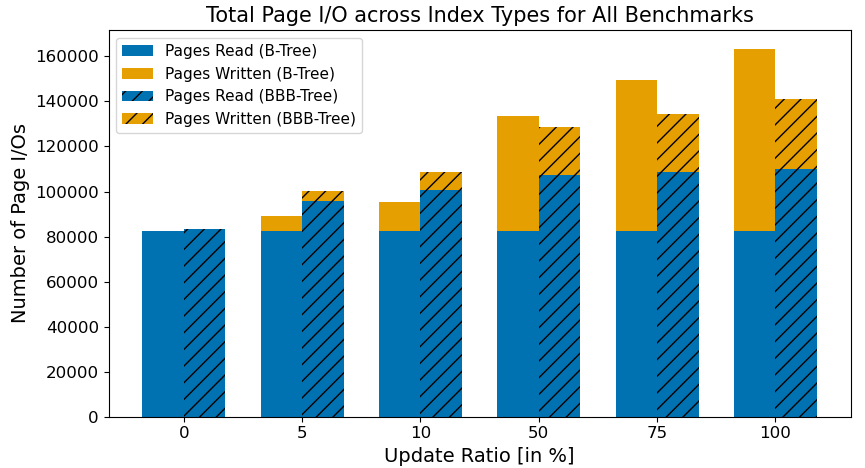
\includegraphics[width=0.7\textwidth]{figures/evaluation/pageviews_total_io_across_update_ratios.png}
    \caption{Total \ac{IO} operations per index, separated into reads and writes with different update ratios in the workload. When we introduce more page reads than we save page writes, we have more total \ac{IO} operations. This benchmark runs with a buffer pool of 200 pages, a page size of 4 KB, and a write threshold of 5\%. The B-tree has 502 nodes.}
  \label{fig:total-io}
\end{figure}

These findings show that the 3B-tree is not always beneficial in every scenario.
While we can reduce write amplification significantly, we introduce read amplification in the process.
Only in workloads where we have enough writes to compensate for the additional reads, we can achieve a net reduction in \ac{IO} operations.

We can express this trade-off in a payoff condition for our method.
Consider a workload consisting of read operations and write operations.
The proposed method amplifies reads by a fraction $read\_amplification$ (expressed as a percentage)  
and reduces writes by a fraction $write\_reduction$ (also in percent).

\begin{equation}
\frac{reads}{writes} < \frac{write\_reduction}{read\_amplification}
\label{eq:ratio_condition}
\end{equation}

With the empirical values $read\_amplification = 33\%$ and $write\_reduction = 62\%$ from the insert workload,  
Equation~\ref{eq:ratio_condition_costs} simplifies to:
\begin{equation}
\frac{reads}{writes} < \frac{62}{33} \approx 1.88
\end{equation}

Hence, the method pays off when the workload exhibits fewer than approximately $1.88$ read operations per write.
For example, in a workload where most pages are written to after being read from disk, we have one read per write most of the time $< 1.88$.
This is the pattern we see in the insert workload for example, building the index from scratch.
Also in update-heavy workloads, we can see such patterns.
For example in the 50\% update workload shown in \autoref{fig:total-io}, we have about 1.6 reads per write, so about 60\% of all read pages are written to before being evicted.
Since $1.6 < 1.88$, we reach a net reduction in \ac{IO} operations.
A scenario where our method performs well. 

Depending on the underlying hardware, read and write operations can have different costs.
In a setting where random writes are significantly more expensive than random reads, as on the M1 Pro's SSD with 512 GB, we could see faster runs in the 3B-tree even in scenarios where we have more total \ac{IO} operations due to a high fraction of read operations but less write operations.
However, some SSDs can be faster in writing than reading.
We can extend this condition to account for different costs of read and write operations.
Let $c_r$ and $c_w$ denote the cost per read and per write, respectively.  

\begin{equation}
\frac{reads}{writes} < \frac{c_w}{c_r} \cdot
\frac{write\_reduction}{read\_amplification}
\label{eq:ratio_condition_costs}
\end{equation}

To summarize, the 3B-tree is beneficial in workloads where the majority of pages are written to after being read from disk, i.e. workloads with a low read-to-write ratio.
To keep read amplification low, we need to be able to cache the Delta Tree effectively in memory.

% Mixed workload, 400 pages in buffer, varying Update Ratio:
% - We consistently have 10\% more total IO.
% - When we lookup only, we have 1\% more IO.
% - We get up to 50\% more page misses on B-tree pages even though the Delta Tree has only 59 nodes at max (100\% updates).
% - Delta Tree is up to 59 nodes.
% - We amplify reads more with 75\% updates.

% Mixed workload, 5\% udpates, varying Buffer Size:
% - We always have about 10\% more total IO. 

% Mixed workload, 5\% updates, 400 Buffer Size, varying Write Threshold:
% - with 0\% write threshold, we have 1\% more total IO, delta tree is 1 node
% - with 1\% write threshold, we have 4\% more total IO, delta tree is 16 nodes
% - with 5\% write threshold, we have 10\% more total IO, delta tree is 32 nodes
% - Why do we have so many delta nodes here? the insert workload operates on the same number of B-tree nodes but generates 19 delta nodes only.
% -> because more nodes produce small deltas in udpates between page swaps. In insertion more change than 5\% happens for most pages.

% Insert workload, varying Buffer Size:
% - With a buffer pool size of 400 we have 13\% less total IO
% - With a buffer pool size of 300 we have 20\% less total IO
% - With a buffer pool size of 200 we have 23\% less total IO
% - With a buffer pool size of 100 we have 17\% less total IO
% - We have enough page writes and less page reads -> net gain
% - Buffer Size does not really matter. We linearly have more/less total IO with smaller/larger buffer sizes.

% Insert workload, varying Write Threshold:
% - With no write threshold, we have 0.37\% more total IO
% - With a write threshold of 1\%, we have 12\% less total IO
% - With a write threshold of 5\%, we have 23\% less total IO
% - With a write threshold of 10\%, we have 17\% less total IO
% - With a write threshold of 15\%, we have 8\% less total IO
% - The higher the write threshold, the more page reads we have -> less net gain.

% We are not good in a scenario with very limited memory, as we constantly swap pages in and out of the buffer pool to perform operations on both trees.
% With more memory, we can cache the Delta Tree pages better, reducing read amplification.
% With too much memory, we amplify the reads too much because the B-tree pages are mostly in memory already, where the Delta Tree hurts more.

\subsection{Space Utilization}
\label{sec:space_overhead}
To track changes we need to store additional metadata in the B-tree nodes.
This introduces a fixed overhead per B-tree node.

\inlinesection{Tracking Modified Entries.}
Firstly, we store the state of each entry in the B-tree node to track whether it has been modified or not.
We inject this information into the slot of each entry.
As mentioned in \autoref{chap:implementation}, we can use 2 bits to encode each state (Unchanged, Inserted, Updated, Deleted).
Since the slot data layout is critical to maximize fanout, we hide this information in the existing slot structure.
We use the two most significant bits of the offset to store the state.

\inlinesection{Tracking Degree of Change of Nodes.}
Secondly, we track the degree of change for each node.
To that end we store a counter in each B-tree node that tracks the approximate number of bytes that have been modified since the last write to disk.
This counter is used to determine whether the write threshold has been reached and the node needs to be written to disk.
We use a 16-bit unsigned integer for this counter, which allows us to track changes up to 65535 bytes.
This is sufficient for our use case, as we can track changes up to 100\% of a 64 KB page.
More realistically though, we do not want to track changes beyond 50\% of a page, therefore we could even track larger page sizes with this counter.

This means that our implementation introduces a fixed overhead of 2 B per node.
However, this does not affect the fanout of the index significantly.
In some scenarios, it does not affect the fanout at all.
For example, assume we store entries of 16 B each (8 B key, 8 B value) on 4 KB pages as we do in our previous benchmarks.
On a leaf node, each entry requires 24 B, a slot of 8 B (4 B offset, 2 B key size, 2 B value size) and the data of 16 B (8 B key, 8 B value).
Therefore, our B-tree leaf nodes can hold 170 entries on a 4 KB page.
With a header of 12 B, a full leaf node occupies $12 B + 170 \cdot 24 B = 4092 B$.
With the additional overhead of 2 B per node, $ 4092 B + 2 B = 4094 B < 4096 B$, we can still fit the same amount of entries on a page.
The same applies to inner nodes.
In this scenario, we do not lose any fanout due to the additional overhead.
However, in other scenarios we might lose one entry per node due to the additional overhead.
With a 4 KB page and 170 entries per node, loosing one entry means a loss of \textasciitilde0.6\% in fanout.

\subsection{In-Memory Overhead}
\label{sec:in-memory-overhead}
To analyze the memory overhead of tracking changes on the pages in memory, we run the mixed Wikipedia Pageviews workload purely in memory, once on a B-tree with tracking enabled and once on a B-tree without tracking.
The B-tree without tracking does not have a Delta Tree attached, so we can see the pure overhead of tracking changes in the B-tree nodes.
We fixate the buffer pool size to 600 pages to ensure that the whole index fits in memory.
This way we can look at the pure memory overhead without the influence of page swaps.
The results are shown in \autoref{tab:tracking-overhead}.
We see that the overhead of tracking changes in memory is negligible.

\begin{table}[ht]
\centering
\begin{tabular}{l|l}
\toprule
\textbf{Index Type} & Time \\
\midrule
\textbf{B-tree without Tracking}  & 13.54 ms \\
\textbf{B-tree with Tracking}  & 13.55 ms (+0.07\%) \\
\bottomrule
\end{tabular}
\caption{Time to insert the Wikipedia Pageviews workload on an empty B-tree with and without tracking changes. The buffer manager fits the whole index in memory. The memory overhead of tracking changes is negligible.}
\label{tab:tracking-overhead}
\end{table}

\subsection{Variable-Sized Entries}
\label{sec:variable-sized-entries}
To analyze the effect of variable-sized entries, we run the same Wikipedia Pageviews workload, but this time with the variable-sized \texttt{page\_title} as key.
As expected, the index size increases due to the larger average key size of \textasciitilde 20.5 B compared to the fixed size keys of 8 B.
We observed that the B-tree has 757 nodes with variable-sized keys compared to 502 nodes with integer keys.
To remove the influence of different index sizes, and therefore more pages, we run the benchmarks with a buffer pool that fits \textasciitilde40\% of the B-tree in memory respectively (300 pages for fixed-sized keys, 200 pages for variable-sized keys).
We run the same workload with 100\% insertions.
The results are shown in \autoref{fig:total-io-variable-size}.

\begin{figure}[htbp]
  \centering
  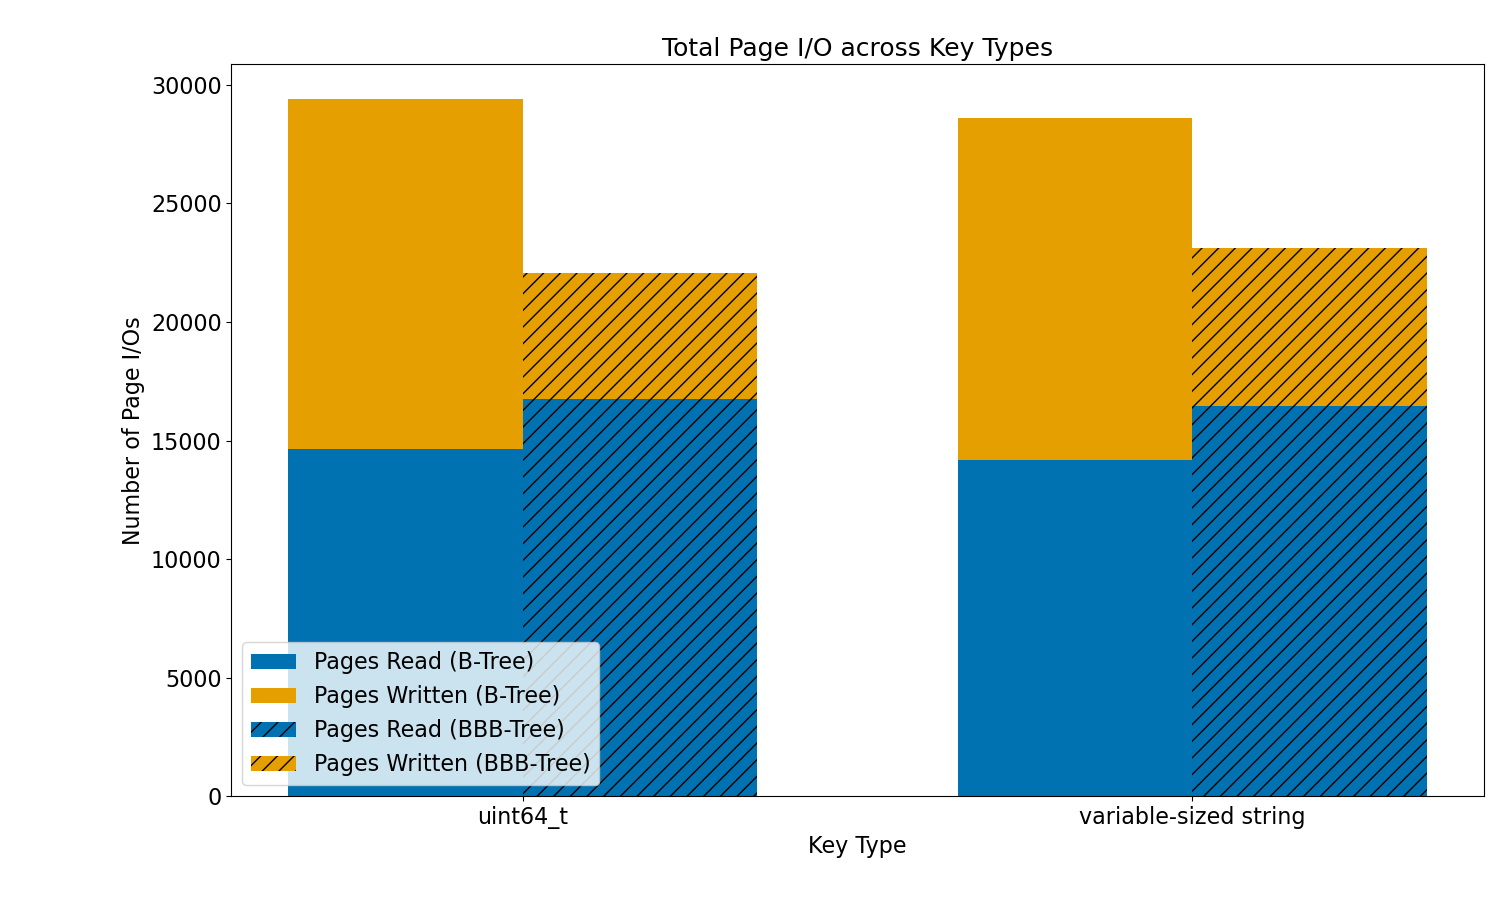
\includegraphics[width=0.9\textwidth]{figures/evaluation/pageviews_total_io_variable_size.png}
  \caption{Total \ac{IO} operations per index, separated into reads and writes with 100\% insertions of variable-sized string keys and fixed-sized integer keys. The buffer pool fits \textasciitilde40\% of the B-tree in memory, the page size is 4 KB and the write threshold is 5\%. While we can reduce total \ac{IO} operations in both cases, the write reduction is smaller with variable-sized keys.}
  \label{fig:total-io-variable-size}
\end{figure}

With the different buffer sizes we achieve similar page reads and writes for the baseline B-trees.
However, with variable-sized keys, the 3B-tree achieves a smaller reduction in page writes compared to fixed-sized keys.
With variable-sized keys, we can reduce page writes by \textasciitilde56\% compared to \textasciitilde64\% with fixed-sized keys.
This has two reasons:
\begin{enumerate}
  \item \textbf{Larger Delta Tree:} 
  With variable-sized keys we generate more B-tree nodes (757 vs 502).
  Therefore, we have more pages that can produce deltas, leading to a larger Delta Tree.
  Our Delta Tree implementation stores the updated entries, therefore variable-sized entries lead to larger deltas as well, increasing the size of the Delta Tree further.
  While both Delta Trees are \textasciitilde3.8\% of the size of their respective B-trees, the Delta Tree is larger in absolute terms.
  A larger Delta Tree leads to more page traffic and therefore more page writes.
  \item \textbf{Larger Modification Degrees:}
  With variable-sized keys, we have more variance in the modification degree of pages as shown in \autoref{tab:modification-degree-variable-size}.
  Therefore, we have less pages with a modification degree below the write threshold of 5\%.
  This leads to less pages being buffered in the Delta Tree and therefore, a smaller overall write reduction.
\end{enumerate}

While a conclusion could be that variable sized keys require a larger write threshold to achieve similar write reductions, we could not confirm this hypothesis with our experiments.
Larger write thresholds lead to larger Delta Trees and no further reduction in write amplification.
To summarize, our method works with variable-sized keys as well, but the write reduction is smaller, mainly due to larger modification degrees of pages.

\begin{table}[ht]
\centering
\begin{tabular}{l|cc}
   \toprule
    & \multicolumn{2}{c}{\textbf{Num. Pages}} \\
    \cmidrule(lr){2-3}
    \textbf{Modified} & \textbf{Fixed-Size Keys} & \textbf{Variable-Size Keys} \\
    \midrule
    0-5     & 12487 & 11013 \\
    5-10    & 2470  & 3303  \\
    10-15   & 64    & 180   \\
    15-20   & 5     & 26    \\
    20-25   & 1     & 4     \\
    25-30   & 0     & 2     \\
    30-35   & 0     & 0     \\
    35-40   & 0     & 1     \\
    40-45   & 0     & 10    \\
    45-50   & 104   & 239   \\
    50-55   & 446   & 477   \\
    55-60   & 59    & 139   \\
    60-65   & 15    & 43    \\
    65-70   & 13    & 23    \\
    70-75   & 11    & 19    \\
    75-80   & 5     & 16    \\
    80-85   & 2     & 13    \\
    85-90   & 7     & 9     \\
    90-95   & 6     & 11    \\
    95-100  & 9     & 13    \\
    >=100   & 109   & 163   \\
    \midrule
    Total Evictions & 15813 & 15705 \\
\bottomrule
\end{tabular}
\caption{Distribution of B-tree pages by their modification degree (percentage intervals) when being evicted with a write threshold of 5\% for fixed-sized keys and variable-sized keys in a workload with 100\% insertions. While both have similar number of page evictions, the variable-sized keys have more variance in the modification degree and less pages with a degree of change below the write threshold of 5\%.}
\label{tab:modification-degree-variable-size}
\end{table}

% \subsection*{Different Page Sizes}

%TODO: Compare performance with sequential updates vs random updates.
